\chapter{Data Aware Workflow Partitioning}
\label{chap:partitioning}

When mapping data-intensive tasks to compute resources, scheduling mechanisms need to take into account not only the execution time of the tasks, but also the overheads of staging the dataset. This also applies to the task clustering problem since merging tasks usually means data transfers associated with these tasks have to be merged as well. In this chapter, we introduce our work on data aware workflow partitioning that divides large scale workflows into several sub-workflows that are fit for execution within a single execution site. Three widely used workflows have been used to evaluate the effectiveness of out methods and the experiments show an runtime improvement of up to 48.1\%. 


\section{Motivation}

Data movement between tasks in scientific workflows has received less attention compared to task execution. Often the staging of data between tasks is either assumed or the time delay in data transfer is considered to be negligible compared to task execution, which is not true in many cases, especially in data-intensive applications. In this chapter, we take the data transfer into consideration and propose to partition large workflows into several sub-workflows where each sub-workflows can be executed within one execution site. 

The motivation behind workflow partitioning starts from a common scenario where a researcher at a research institution typically has access to several research clusters, each of which may consist of a small number of nodes. The nodes in one cluster may be very different from those in another cluster in terms of file system, execution environment, and security systems. For example, we have access to FutureGrid \cite{FutureGrid}, Teragrid/XSEDE \cite{TeraGrid}  and Amazon EC2 \cite{AmazonAWS} but each cluster imposes a limit on the resources, such as the maximum number of nodes a user can allocate at one time or the maximum storage. If these isolated clusters can work together, they collectively become more powerful.

Additionally, the input dataset could be very large and widely distributed across multiple clusters. Data-intensive workflows require significant amount of storage and computation and therefore the storage system becomes a bottleneck. For these workflows, we need to use multiple execution sites and consider their available storage. For example, the entire CyberShake earthquake science workflow has 16,000 sub-workflows and each sub-workflow has more than 24,000 individual jobs and requires 58 GB of data. In this chapter, we assume we have Condor installed at the execution sites. A Condor pool can be either a physical cluster or a virtual cluster. 

The first benefit of workflow partitioning is that this approach reduces the complexity of workflow mapping. For example, the entire CyberShake workflow has more than $3.8\times 10^8$ tasks, which is a significant load for workflow management tools to maintain or schedule. In contrast, each sub-workflow has 24,000 tasks, which is acceptable for workflow management tools. A sub-workflow is a workflow and also a job of a higher-level workflow. What is more, workflow partitioning provides a fine granularity adjustment of workflow activities so that each sub-workflow can be adequate for one execution site. In the end, workflow partitioning allows us to migrate or retry sub-workflows efficiently. The overall workflow can be partitioned into sub-workflows and each sub-workflow can to be executed in different execution environments such as a hybrid platform of Condor/DAGMan \cite{DAGMan} and MPI/DAGMan \cite{Rynge2012}) while the traditional task clustering technique requires all the tasks can be executed in the same execution environment. 


%should fix it

 
%There are large differences in I/O speeds from local disk storage to wide area networks. Feeding a large dataset repeatedly to re- mote computing resources becomes the bottleneck. When mapping such data-intensive tasks to compute resources, scheduling mechanisms need not only take into account the execution time of the tasks, but also the overheads of staging the dataset. To scale up such tasks, there are tradeoffs to be made, such as determining whether to bring data to computation or bring computation to data, or even regenerate data on-the-fly.

%While scheduling workflows there exists more than one task that can be scheduled independently of one another. Since our workflows are data intensive in nature, the transfer time are dominant as compared to the computation time. This gives rise to the possibility that majority of tasks are assigned to a single or only few compute resources. This occurs only when tasks have more than one input file in common and these files are only available from selected few resources. In such cases, grouping these tasks to form a batch task and submitting to a resource reduces data-transfer time.

%\section{Related Work}
%For convenience and cost-related reasons, scientists execute scientific workflows \cite{Bharathi2008, Rubing2005} in distributed large-scale computational environments such as multi-cluster grids, that is, grids comprising multiple independent execution sites. Topcuoglu \cite{Topcuoglu2002} presented a classification of widely used task scheduling approaches. Such scheduling solutions, however, cannot be applied directly to multi-cluster grids. First, the data transfer delay between multiple execution sites is more significant than that within an execution site and thus a hierarchical view of data transfer is necessary. Second, they do not consider the resource availability experienced in grids, which also makes accurate predictions of computation and communication costs difficult. Sonmez \cite{Sonmez2010} extended the traditional scheduling problem to multiple workflows on multi-cluster grids and presented a performance of a wide range of dynamic workflow scheduling policies in multi-cluster grids. Duan \cite{Rubing2005} and Wieczorek \cite{Wieczorek2005} have discussed the scheduling and partitioning scientific workflows in dynamic grids with challenges such as a broad set of unpredictable overheads and possible failures. Duan \cite{Rubing2005} then developed a distributed service-oriented Enactment Engine with a master-slave architecture for de-centralized coordination of scientific workflows. Kumar \cite{Kumar2002} proposed the use of graph partitioning for partition the resources of a distributed system, but not the workflow DAG, which means the resources are provisioned into different execution sites but the workflows are not partitioned at all. Dong \cite{Dong2007} and Kalayci \cite{Kalayci2010} have discussed the use of graph partitioning algorithms for the workflow DAG according to features of the workflow itself and the status of selected available resource clusters. Our work focuses on the workflow partitioning problem with resource constraints. Compared to Dong \cite{Dong2007} and Kalayci \cite{Kalayci2010}, we extend their work to estimate the overall runtime of sub-workflows and then schedule these sub-workflows based on the estimates. 

%Yu \cite{Yu2005a} classified existing automated data transfer strategies utilized among tasks in workflows, namely centralized, mediated, and peer-to-peer. A centralized approach utilizes a central point for data transmission. This solution is not scalable, and occurs in systems where the time for data transfers is much smaller than computations. Taverna \cite{Oinn2004} typically utilizes a centralized data transfer, due to the characteristics of the problems it tackles. In a mediated strategy the locations of the intermediate data are managed by a distributed data management system. Finally, a peer-to-peer approach transfers data directly between processing nodes. The direct transmissions of peer-to-peer approaches reduce both transmission time and the bottleneck problem caused by the centralized and mediated approaches. Thus, they are suitable for large-scale intermediate data transfer. For simplicity, we use centralized data services but our work can be easily extended to the peer-to-peer approach with modifications. 

%The Pegasus workflow system [7] has also dealt with data-intensive workflows and has incorporated both mediated and peer-to-peer transfers. In the mediated approach, Pegasus utilises a data replica catalogue that stores the intermediate data generated, so data can be subsequently retrieved rather than recomputed again. Workflow performance speedup has also been a matter of study in Pegasus, and abstract workflow specifications go through a process of clustering (grouping of small tasks) and partitioning which helps the meta-scheduler to optimise the execution time. A similar approach was followed in \cite{Rubing2005} with further optimisation at runtime by adapting to the dynamically changing state of underlying resources. However, none of these approaches makes an effective usage of both network bandwidth and buffer/storage of files.

%Park et al. \cite{Humphrey2008} limits the amount of parallel data transfer to avoid overloading supporting services such as data servers, which is called data throttling. Throttling is especially useful for unbalanced workflows in which one task might be idle while waiting for data to arrive. However, as discussed in \cite{Humphrey2008}, data throttling has an impact on the overall workflow performance depending on the ratio between computational and data transfer tasks. Therefore, performance analysis is necessary after the profiling of data transfers so that the relationship between computation and data transfers can be identified more explicitly. Rodríguez \cite{Rodríguez2012} proposed an automated and trace-based workflow structural analysis method for DAGs. Files transfers are accomplished as fast as the network bandwidth allows, and once transferred, the files are buffered/stored at their destination. To improve the use of network bandwidth and buffer/storage within a workflow, they adjusted the speeds of some data transfers and assured that tasks have all their input data arriving at the same time. Compared to our work, data throttling has a limit in performance gain by the amount of data transfer that can be reduced, while our partitioning approach can improve the overall workflow runtime and resource usage. 

%Data Placement techniques try to strategically manage placement of data before or during the execution of a workflow. Kosar et al. \cite{Kosar2004} presented Stork, a scheduler for data placement activities on grids and proposed to make data placement activities as first class citizens in the Grid. In Stork, data placement is a job and is decoupled from computational jobs. Amer et al. \cite{Amer2012} studied the relationship between data placement services and workflow management systems for data-intensive applications. They proposed an asynchronous mode of data placement in which data placement operations are performed as data sets become available and according to the policies of the virtual organization and not according to the directives of the workflow management system (WMS). The WMS can however assist the placement services with the placement of data based on information collected during task executions and data transfers. Shankar \cite{Shankar2007} presented an architecture for Condor in which the input, output and executable files of jobs are cached on the local disks of the machines in a cluster. Caching can reduce the amount of pipelines and batch I/O that is transferred across the network. This in turn significantly reduces the response time for workflows with data-intensive workloads. In contrast, we mainly focus on the workflow partitioning problem but our work can be extended to consider the data placement strategies they have proposed in the future. 

%With caching enabled, data-intensive applications can reuse the files and also be able to compare between old and new versions of the file. They presented a planning algorithm that takes into account the location of cached data together with data dependencies between jobs in a workflow. Their planning algorithm produces a schedule by comparing the time saved by running jobs in parallel with the time taken for transferring data when dependent jobs are scheduled on different machines. 

%Data replication is a common way to increase the availability of data and implicit replication also occurs when scientists download and share the data for experimental purposes, in contrast to explicit replications done by workflow systems. Ranganathan  \cite{Ranganathan2001} conducted extensive studies for identifying dynamic data or task replication strategies, asynchronous data placement and job and data scheduling algorithms for Data Grids. They concluded through simulations of independent jobs that scheduling jobs to locations that contain the data they need and asynchronously replicating popular data sets to remote sites can improve the performance. We do not address data replication in our current work but it is worthy of further investigation of how data replication can improve the performance of workflow partitioning. 

%Their replication process at each site periodically generates new replicas for popular datasets. For dataset placement scheduler they define three algorithms: Data- DoNothing- no active replication takes place, DataRandom- popular datasets are replicated to a random site on the Grid, DataLeastLoaded- popular datasets are replicated to a least loaded neighboring site. 

%In data-intensive applications, replication may or may not be feasible. 

\section{Approach}

To efficiently partition workflows, we proposed a three-phase scheduling approach integrated with the Pegasus Workflow Management System to partition, estimate, and schedule workflows onto distributed resources. Our contribution includes three heuristics to partition workflows respecting storage constraints and internal job parallelism. We utilize three methods to estimate and compare runtime of sub-workflows and then we schedule them based on two commonly used algorithms (MinMin and HEFT).  

\begin{figure}[lh!]
	\centering
    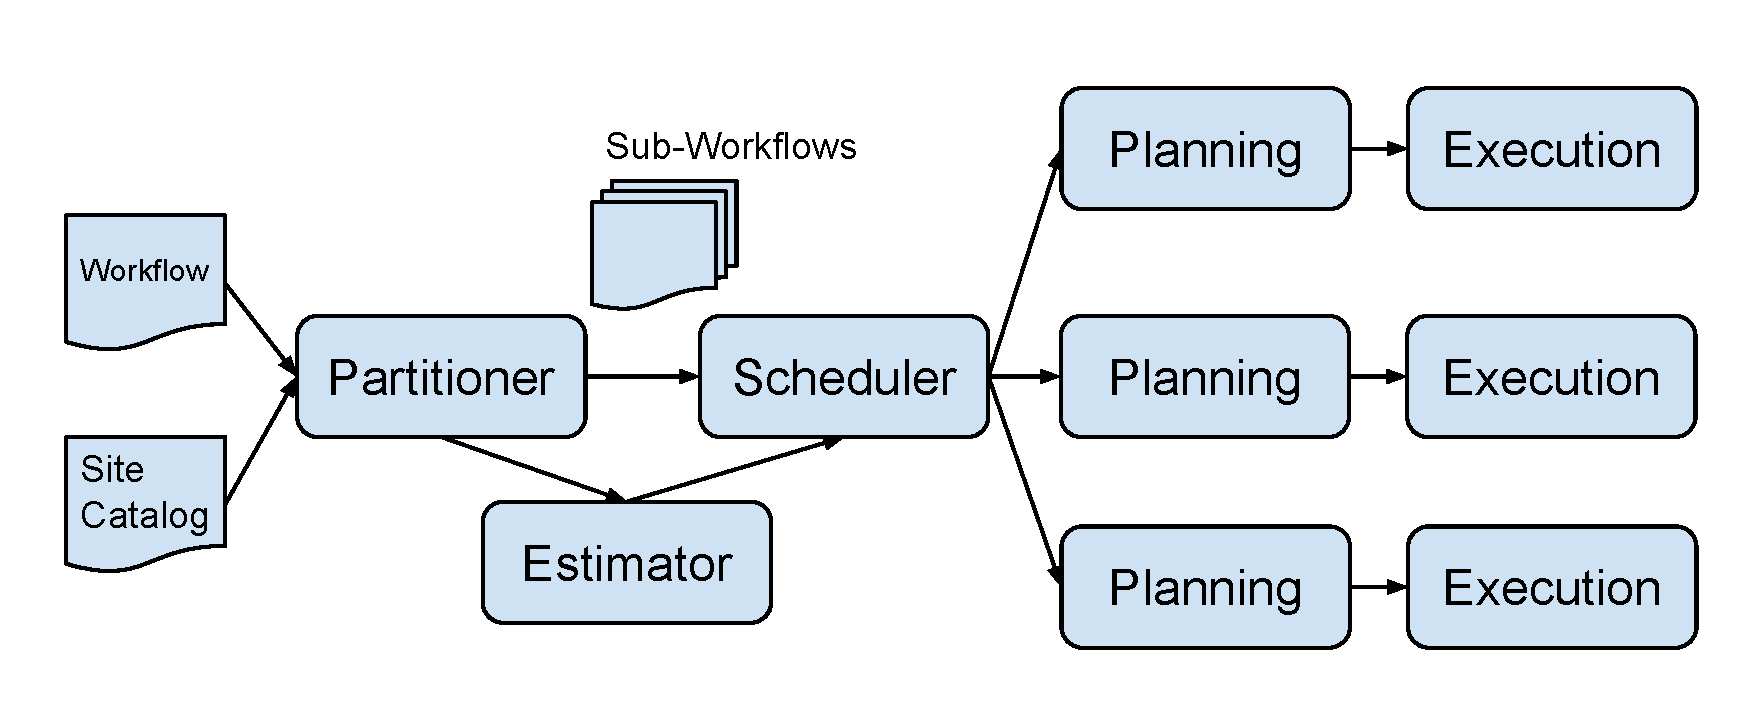
\includegraphics[width=0.8\textwidth]{figures/partitioning/partitioning_steps.pdf}
    \caption{The steps to partition and schedule a workflow}
    \label{fig:partitioning_steps}
\end{figure}
\begin{figure}[lh!]
	\centering
    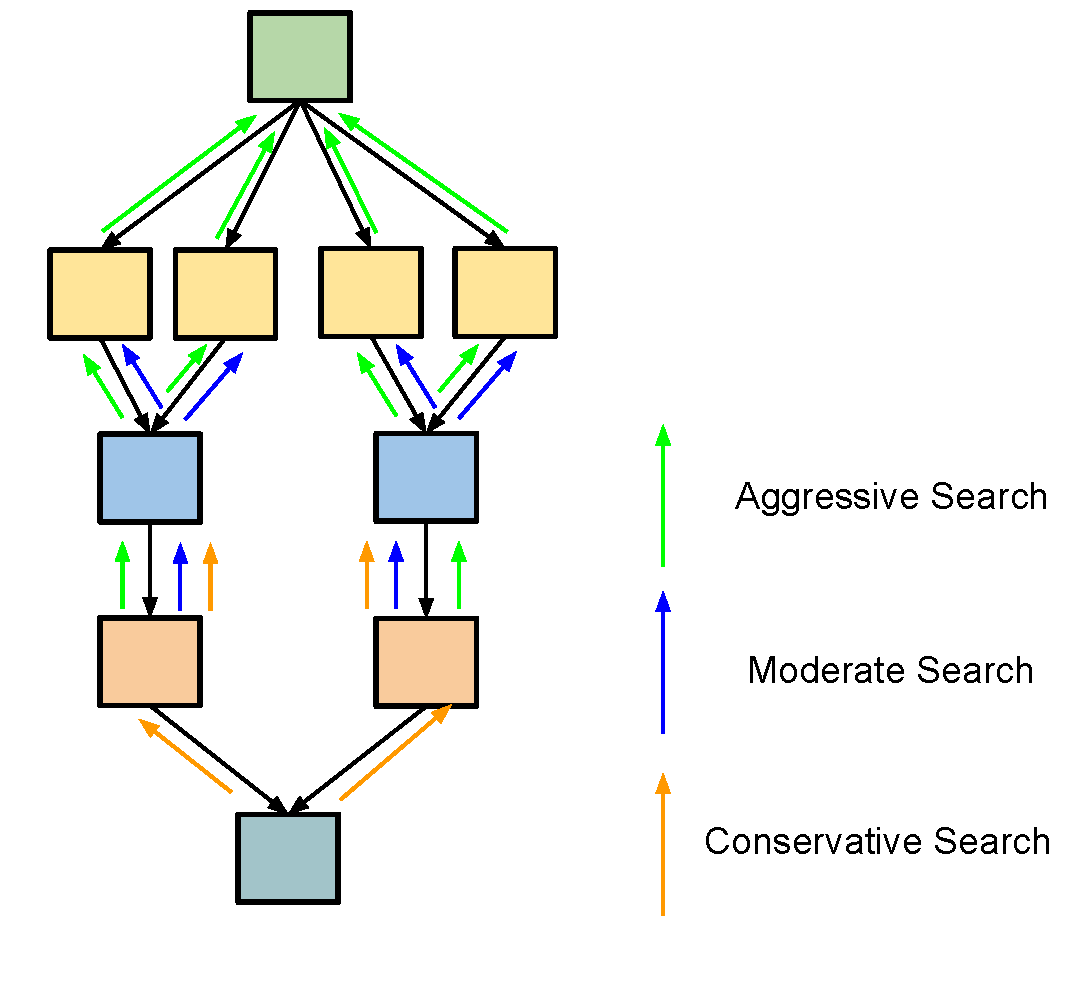
\includegraphics[width=0.7\textwidth]{figures/partitioning/three_steps.pdf}
    \caption{Three Steps of Search}
    \label{fig:three_steps}
\end{figure}
\begin{figure}[lh!]
	\centering
    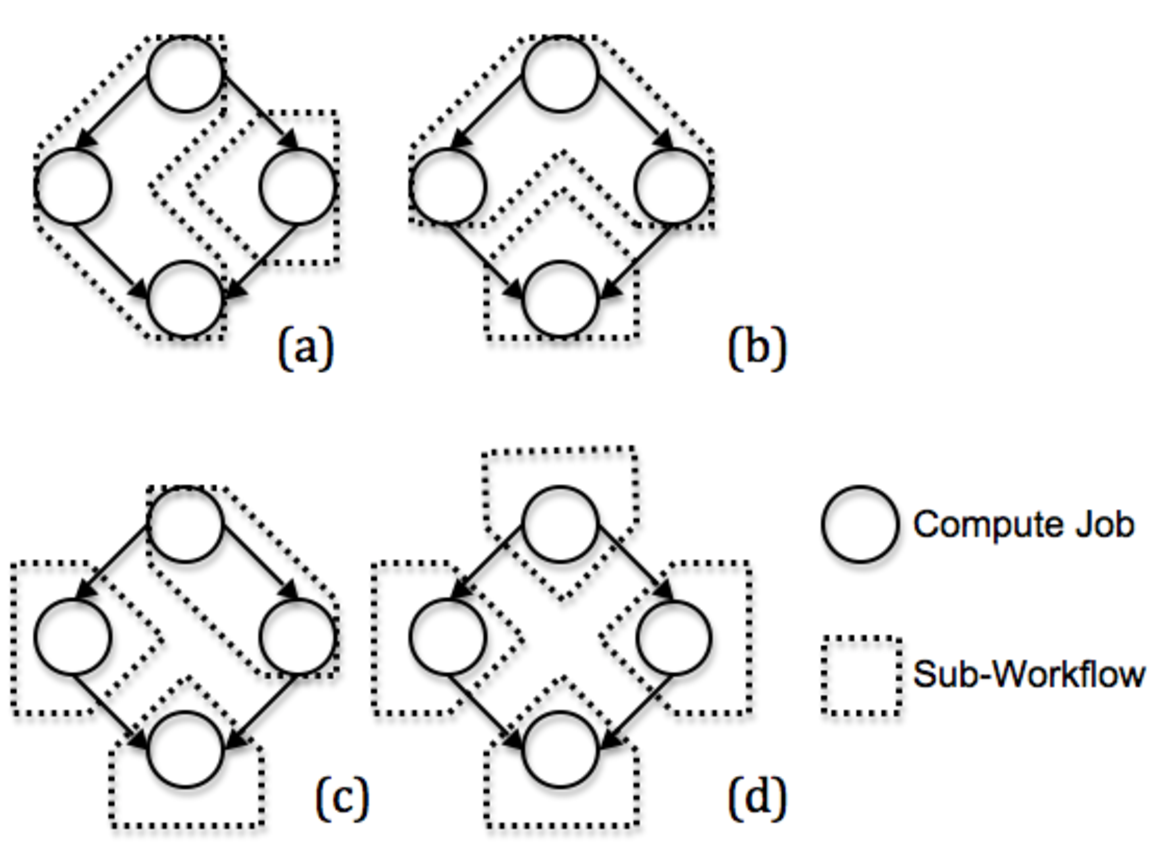
\includegraphics[width=0.9\textwidth]{figures/partitioning/four_partitioning.pdf}
    \caption{Four Partitioning Methods}
    \label{fig:four_partitioning}
\end{figure}
Our approach (see Figure~\ref{fig:partitioning_steps}) has three phases: partition, estimate and schedule. The partitioner takes the original workflow and site catalog as input, and outputs various sub-workflows that respect the storage constraints—this means that the data requirements of a sub-workflow are within the data storage limit of a site. The site catalog provides information about the available resources. The estimator provides the runtime estimation of the sub-workflows and supports three estimation methods. The scheduler maps these sub-workflows to resources considering storage requirement and runtime estimation. The scheduler supports two commonly used algorithms. We first guarantee to find a valid mapping of sub-workflows satisfying storage constraints. Then we optimize performance based on these generated sub-workflows and schedule them to appropriate execution sites if runtime information for individual jobs is already known. If not, a static scheduler maps them to resources merely based on storage requirements. 

The major challenge in partitioning workflows is to avoid cross dependency, which is a chain of dependencies that forms a cycle in graph (in this case cycles between sub-workflows). With cross dependencies, workflows are not able to proceed since they form a deadlock loop. For a simple workflow depicted in Figure~\ref{fig:four_partitioning}, we show the result of four different partitioning. Partitioning (a) does not work in practice since it has a deadlock loop. Partitioning (c) is valid but not efficient compared to Partitioning (b) or (d) that have more parallelism. 

Usually jobs that have parent-child relationships share a lot of data since they have data dependencies. It’s reasonable to schedule such jobs into the same partition to avoid extra data transfer and also to reduce the overall runtime. Thus, we propose Heuristic I to find a group of parents and children. Our heuristic only checks three particular types of nodes: the fan-out job, the fan-in job, and the parents of the fan-in job and search for the potential candidate jobs that have parent-child relationships between them. The check operation means checking whether one particular job and its potential candidate jobs can be added to a sub-workflow while respecting storage constraints. Thus, our algorithm reduces the time complexity of check operations by n folds, while n is the average depth of the fan-in-fan-out structure. The check operation takes more time than the search operation since the calculation of data usage needs to check all the data allocated to a site and see if there is data overlap. Similar to \cite{Topcuoglu2002}, the algorithm starts from the sink job and proceeds upward. 

To search for the potential candidate jobs that have parent-child relationships, the partitioner tries three steps of searches. For a fan-in job, it first checks if it’s possible to add the whole fan structure into the sub-workflow (aggressive search). If not, similar to Figure~\ref{fig:four_partitioning}(d), a cut is issued between this fan-in job and its parents to avoid cross dependencies and increase parallelism. Then a less aggressive search is performed on its parent jobs, which includes all of its predecessors until the search reaches a fan-out job. If the partition is still too large, a conservative search is performed, which includes all of its predecessors until the search reaches a fan-in job or a fan-out job. Figure~\ref{fig:three_steps} depicts an example of three steps of search while the workflow in it has an average depth of 4. Pseudo-code of Heuristic I is depicted in Algorithm~\ref{alg:parworkflow} .

%The partitioner starts by picking an execution site from site catalog and forming a sub-workflow with the heuristic above. Users must specify the order of execution sites to be picked. If the execution site does not have sufficient storage to host any more jobs, a new execution site is selected and so on. For the dependencies between jobs across multiple sub-workflows, they form the new dependencies between sub-workflows and are added to the final graph. The partitioner guarantees to satisfy storage constraints since in each step it assures the size of all sub-workflows assigned to a site is smaller than its storage constraint. 

We propose two other heuristics to solve the problem of cross dependency. The motivation for Heuristic II is that Partitioning (c) in Figure~\ref{fig:four_partitioning} is able to solve the problem. The motivation for Heuristic III is an observation that partitioning a fan structure into multiple horizontal levels is able to solve the problem. Heuristic II adds a job to a sub-workflow if all of its unscheduled children can be added to that sub-workflow without causing cross dependencies or exceed the storage constraint. Heuristic III adds a job to a sub-workflow if two conditions are met: 
\begin{enumerate}
\item For a job with multiple children, each child has already been scheduled.
\item After adding this job to the sub-workflow, the data size does not exceed the storage constraint.  
\end{enumerate}

To optimize the workflow performance, runtime estimation for sub-workflows is required assuming runtime information for each job is already known. We provide three methods. 
\begin{enumerate}
\item Critical Path is defined as the longest depth of the sub-workflow weighted by the runtime of each job. 
\item Average CPU Time is the quotient of cumulative CPU time of all jobs divided by the number of available resources (it’s the number of Condor slots in our experiments, which is also the maximum number of Condor jobs that can be run on one machine). \item The HEFT estimator uses the calculated earliest finish time of the last sink job as makespan of sub-workflows assuming that we use HEFT to schedule sub-workflows. 
\end{enumerate}

\begin{algorithm}[h!]
\caption{Workflow Partitioning algorithm}
\label{alg:parworkflow}
\begin{algorithmic}[1]
\Require $G$: workflow; $SL[index]$: site list, which stores all information about a compute site
\Ensure Create a subworkflow list $SWL$ that does not exceed storage constraints
\Procedure{ParWorkflow}{$G, SL$}
   \State $index\gets 0$
   \State $Q\gets$ new Queue()
   \State Add the sink job of $G$ to $Q$
   \State $S\gets$ new subworkflow()
   \While{$Q$ is not empty}
      \State $j\gets$ the last job in $Q$
      \State \Call{Aggressive-Search}{$j$} \Comment{for fan-in job}
      \State $C\gets$ the list of potential candidate jobs to be added to $S$ in $SL[index]$
      \State $P\gets$ the list of parents of all candidates
      \State $D\gets$ the data size in $SL[index]$ with $C$
      \If{$D>$ storage constraint of $SL[index]$}
         \State \Call{Less-Aggressive-Search}{j}, update $C,P,D$
      
      \If{$D>$ storage constraint of $SL[index]$}
         \State \Call{Conservative-Search}{j}, update $C,P,D$
      \EndIf
      \EndIf
	\State ...\Comment{for other jobs}
         \If{$S$ causes cross dependency in $SL[index]$}
         \State$S=$ new subworkflow()
      \EndIf
     \State Add all jobs in $C$ to $S$
     \State Add all jobs in $P$ to the head of $Q$
     \State Add $S$ to $SWL[index]$
     \If{$S$ has no enough space left}
         \State $index++$
      \EndIf
   \State ... \Comment{for other situations}
   \State Remove $j$ from $Q$
   \EndWhile
   \State \textbf{return }$SWL$

\EndProcedure
\end{algorithmic}
\end{algorithm}


The scheduler selects appropriate resources for the sub-workflows satisfying the storage constraints and optimizes the runtime performance. Since the partitioning step has already guaranteed that there is a valid mapping, this step is called re-ordering or post-scheduling. We select HEFT\cite{Topcuoglu2002} and MinMin\cite{Blythe2005}, which represent global and local optimizations respectively. But there are two differences compared to their original versions. First, the data transfer cost within a sub-workflow is ignored since we use a shared file system in our experiments. Second, the data constraints must be satisfied for each sub-workflow. 
The scheduler selects an optimal set of resources in terms of available Condor slots since it’s the major factor influencing the performance. This work can be easily extended to considering more factors. Although some more comprehensive algorithms can be adopted, HEFT or MinMin are able to find an optimal schedule in terms that the sub-workflows are already generated since the number of sub-workflows has been greatly reduced compared to the number of individual jobs.

\section{Experiments and Discussion}
In order to quickly deploy and reconfigure computational resources, we use a private cloud computing resource running Eucalyptus \cite{Nurmi2008b}. Eucalyptus is an infrastructure software that provides on-demand access to Virtual Machine (VM) resources. In all the experiments, each VM has 4 CPU cores, 2 Condor slots, 4GB RAM and has a shared file system mounted to make sure data staged into a site is accessible to all compute nodes. In the initial experiments we build up four clusters, each with 4 VMs, 8 Condor slots. In the last experiment of site selection, the four virtual clusters are reconfigured and each cluster has 4, 8, 10 and 10 Condor slots respectively. The submit host that performs workflow planning and which sends jobs to the execution sites is a Linux 2.6 machine equipped with 8GB RAM and an Intel 2.66GHz Quad CPUs. We use Pegasus to plan the workflows and then submit them to Condor DAGMan \cite{DAGMan}, which provides the workflow execution engine. Each execution site contains a Condor pool and a head node visible to the network. 

\begin{figure}[h!]
	\centering
    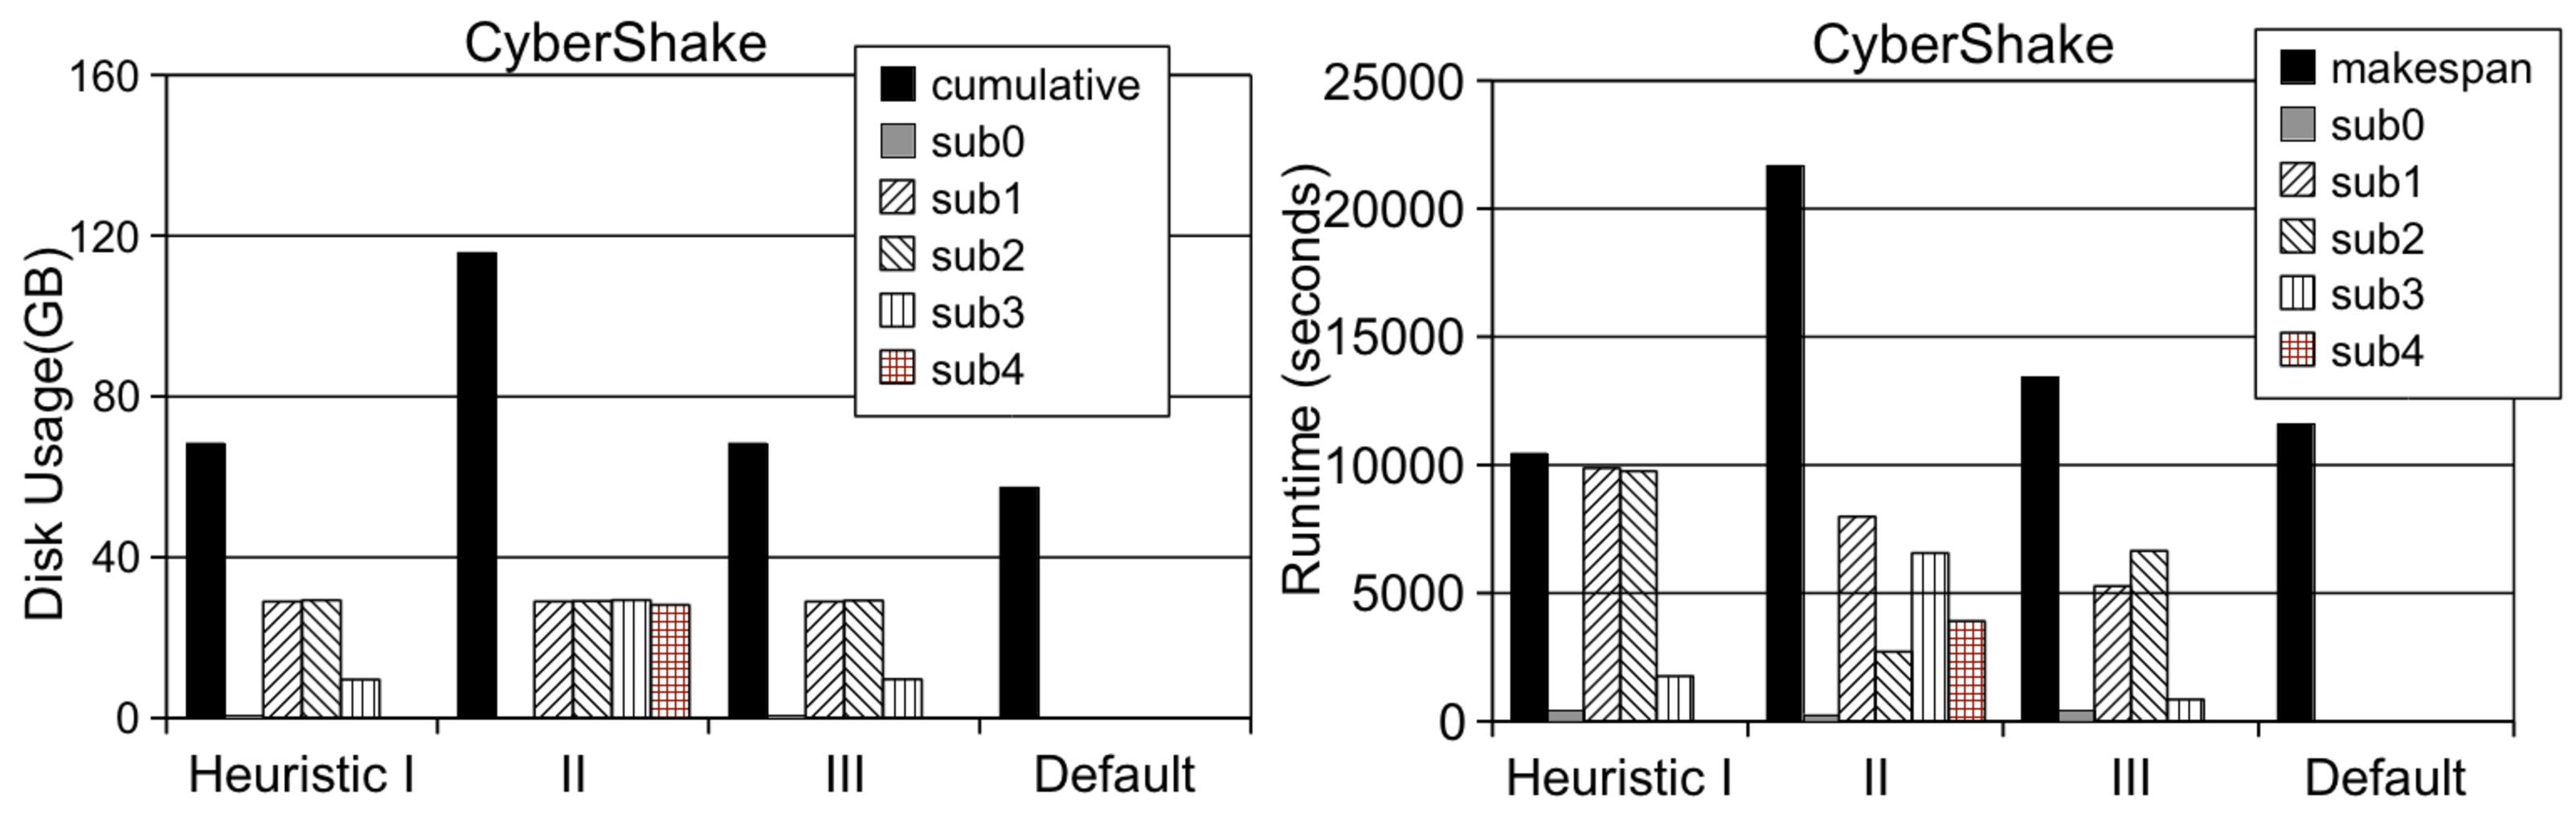
\includegraphics[width=0.9\textwidth]{figures/partitioning/heuristics.pdf}
    \caption{Performance of the three heuristics. The default workflow has one execution site with 4 VMs and 8 Condor slots and has no storage constraint.}
    \label{fig:heuristics}
\end{figure}

%\begin{figure}[h!]
%	\centering
%    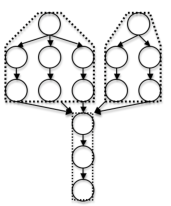
\includegraphics[width=0.3\textwidth]{figures/partitioning/heuristicsI.pdf}
% 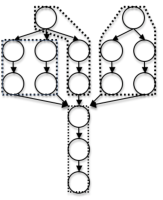
\includegraphics[width=0.3\textwidth]{figures/partitioning/heuristicsII.pdf}
% 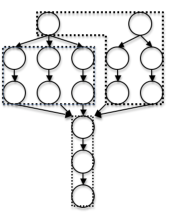
\includegraphics[width=0.3\textwidth]{figures/partitioning/heuristicsIII.pdf}
%    \caption{From left to right: Heuristic I, Heuristic II, Heuristic III.}
%    \label{fig:three_heuristics}
%\end{figure}





\begin{figure}[h!]
	\centering
    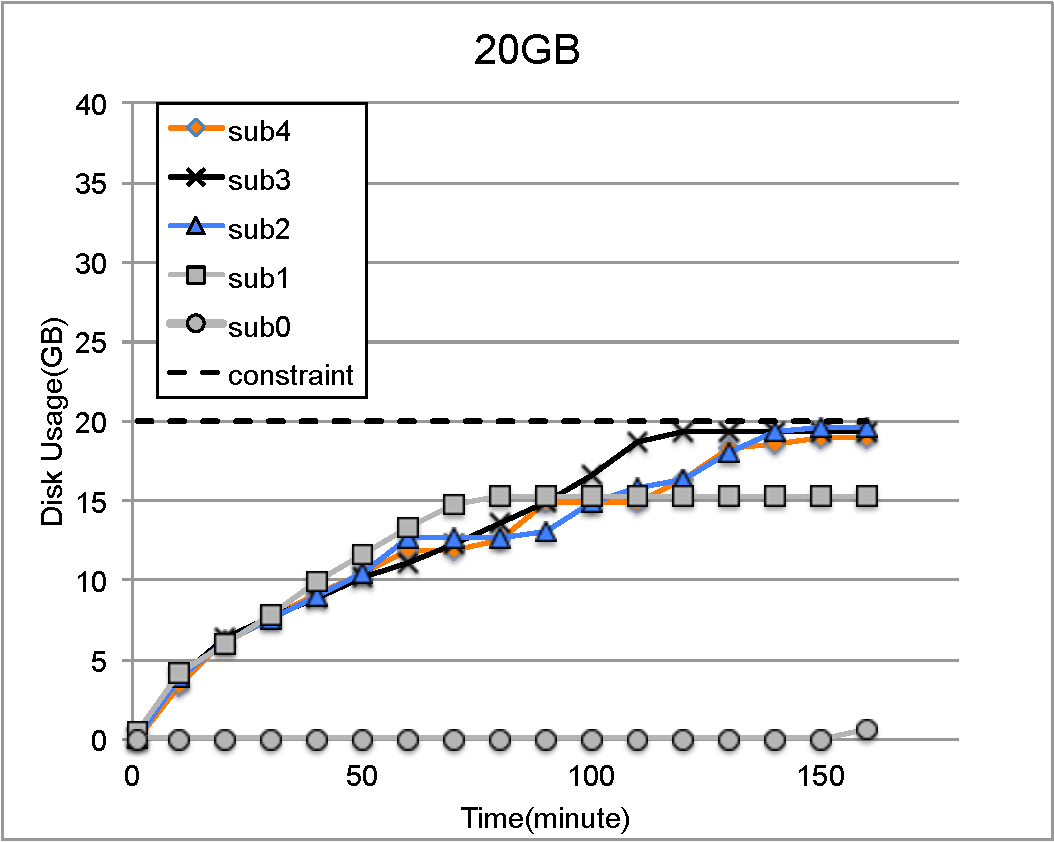
\includegraphics[width=0.49\textwidth]{figures/partitioning/cybershake20gb.pdf}
 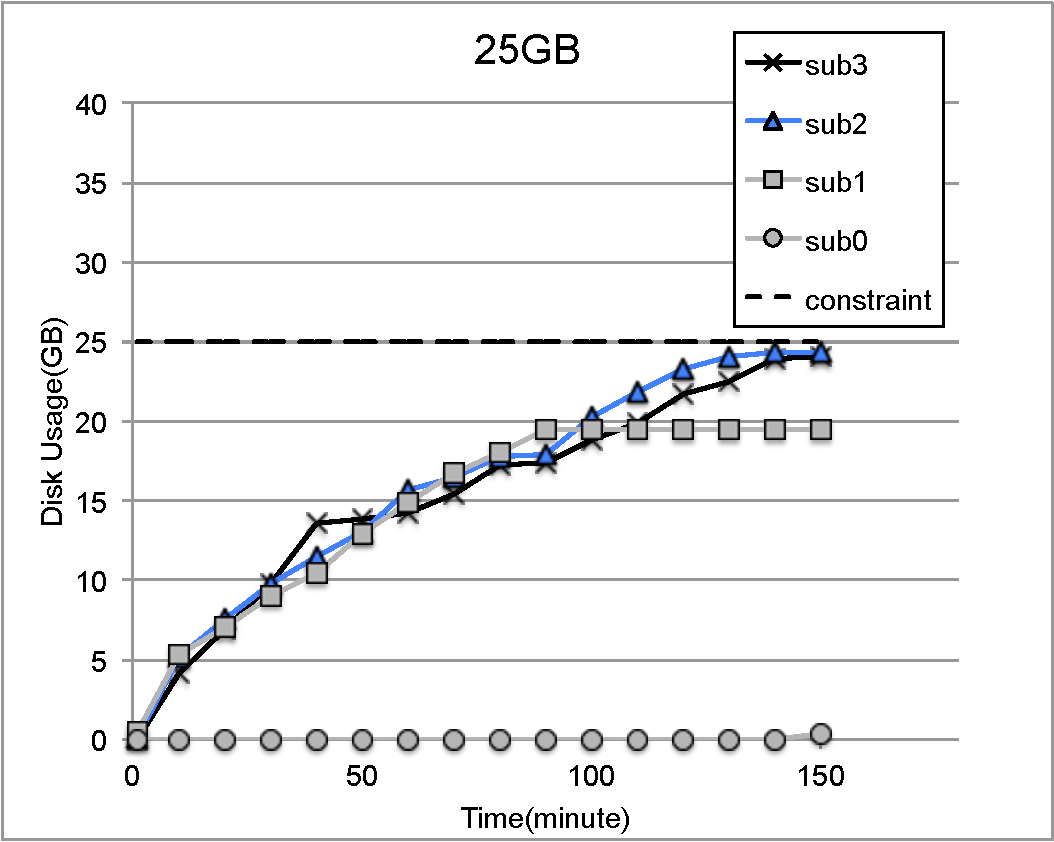
\includegraphics[width=0.49\textwidth]{figures/partitioning/cybershake25gb.pdf}
 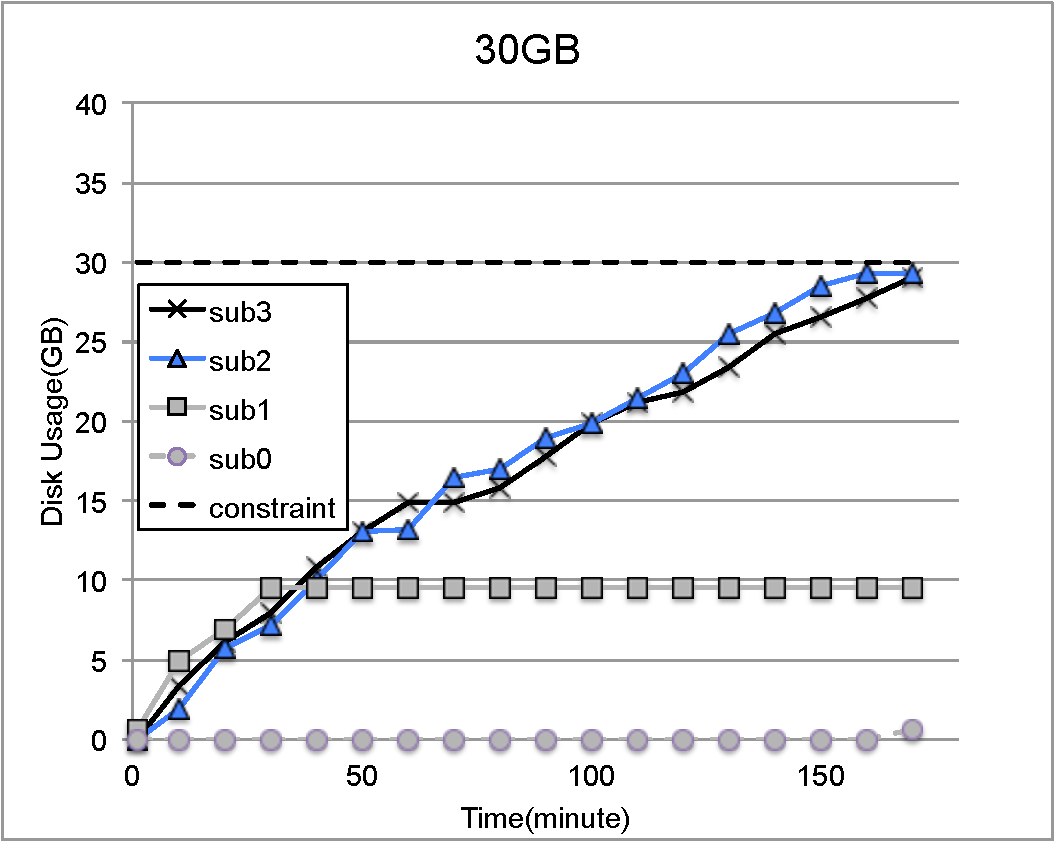
\includegraphics[width=0.49\textwidth]{figures/partitioning/cybershake30gb.pdf}
 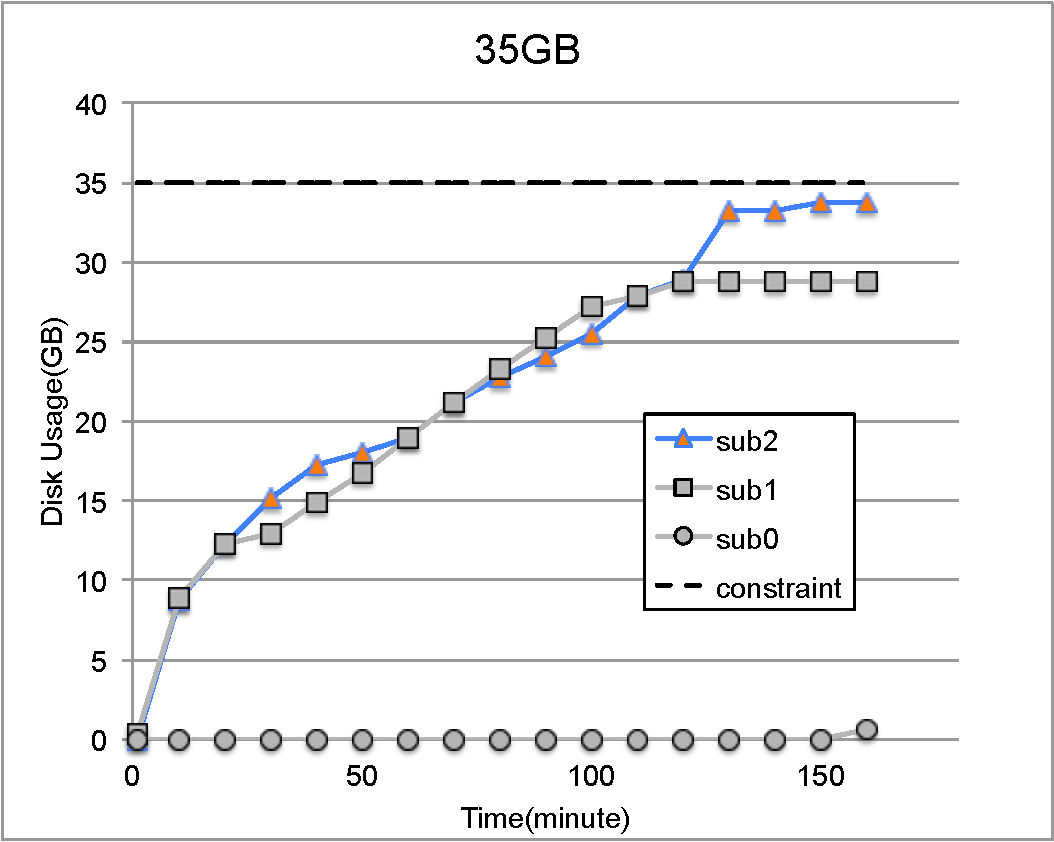
\includegraphics[width=0.49\textwidth]{figures/partitioning/cybershake35gb.pdf}
    \caption{CyberShake with storage constraints of 35GB, 30GB, 25GB, and 20GB. They have 3, 4, 4, and 5 sub-workflows and require 2, 3, 3, and 4 sites to run respectively. }
    \label{fig:constraint}
\end{figure}

\begin{table}[h!]
\caption{CyberShake with Storage Constraint}
\label{tab:constraint}
\centering
\begin{tabular}{lrrrr}
\hline
 storage constraint    &    site &    Disk Usage(GB) &   Percentage  \\
\hline
35GB & A & sub0:0.06; sub1:33.8 & 97\%&\\
& B & sub2:28.8&82\% &\\
30GB & A & sub0:0.07;sub1:29.0 & 97\% \\
& B & sub2:29.3&98\% &\\
& C & sub3:28.8&96\% &\\
25GB & A & sub0:0.06;sub1:24.1 & 97\%& \\

 & B & sub2:24.4 & 98\%& \\
&C&sub3:19.5&78\%&\\
20GB&A&sub0:0.06;sub1:18.9&95\%&\\
&B&sub2:19.3&97\%&\\
&C&sub3:19.6&98\%&\\
&D&sub4:15.3&77\%&\\
\hline
\end{tabular}
\end{table} 


\textbf{Performance Metrics.} To evaluate the performance, we use two types of metrics. Satisfying the Storage Constraints is the main goal of our work in order to fit the sub-workflows into the available storage resources. We compare the results of different storage constraints and heuristics. Improving the Runtime Performance is the second metric that is concerned with in order to minimize the overall makespan. We compare the results of different partitioners, estimators and schedulers. 

\textbf{Workflows Used}. We ran three different workflow applications: an astronomy application (Montage), a seismology application (CyberShake) and a bioinformatics application (Epigenomics). They were chosen because they represent a wide range of application domains and a variety of resource requirements \cite{Juve2009}. 
%For example, Montage is I/O intensive, CyberShake is memory intensive, and Epigenomics is CPU intensive. The goal of the CyberShake Project \cite{Maechling2007} is to calculate Probabilistic Seismic Hazard curves for several geographic sites in the Southern California area. We ran one partition in our experiments that has 24,132 tasks and 58GB of overall data. Montage \cite{Berriman2004} is an astronomy application that is used to construct large image mosaics of the sky. We ran a Montage workflow with a size of 8 degree square of sky. The workflow has 10,422 tasks and 57GB of overall data. Epigenomics \cite{Epigenome} maps short DNA segments collected with high-throughput gene sequencing machines to a reference genome. The workflow has 1,586 tasks and 23GB of overall data. We ran each workflow instance 5 times to account for system variability. 


%\begin{figure}[h!]
%	\centering
%    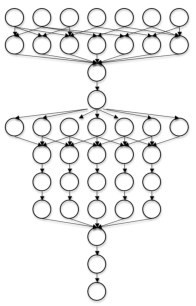
\includegraphics[width=0.3\textwidth]{figures/partitioning/montage.pdf}
%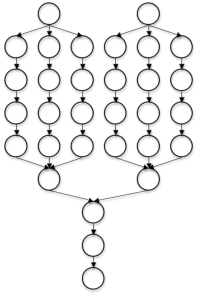
\includegraphics[width=0.3\textwidth]{figures/partitioning/epigenomics.pdf}
%    \caption{The Montage workflow and the Epigenomics workflow}
%    \label{fig:workflow}
%\end{figure}

\begin{figure}[h!]
	\centering
    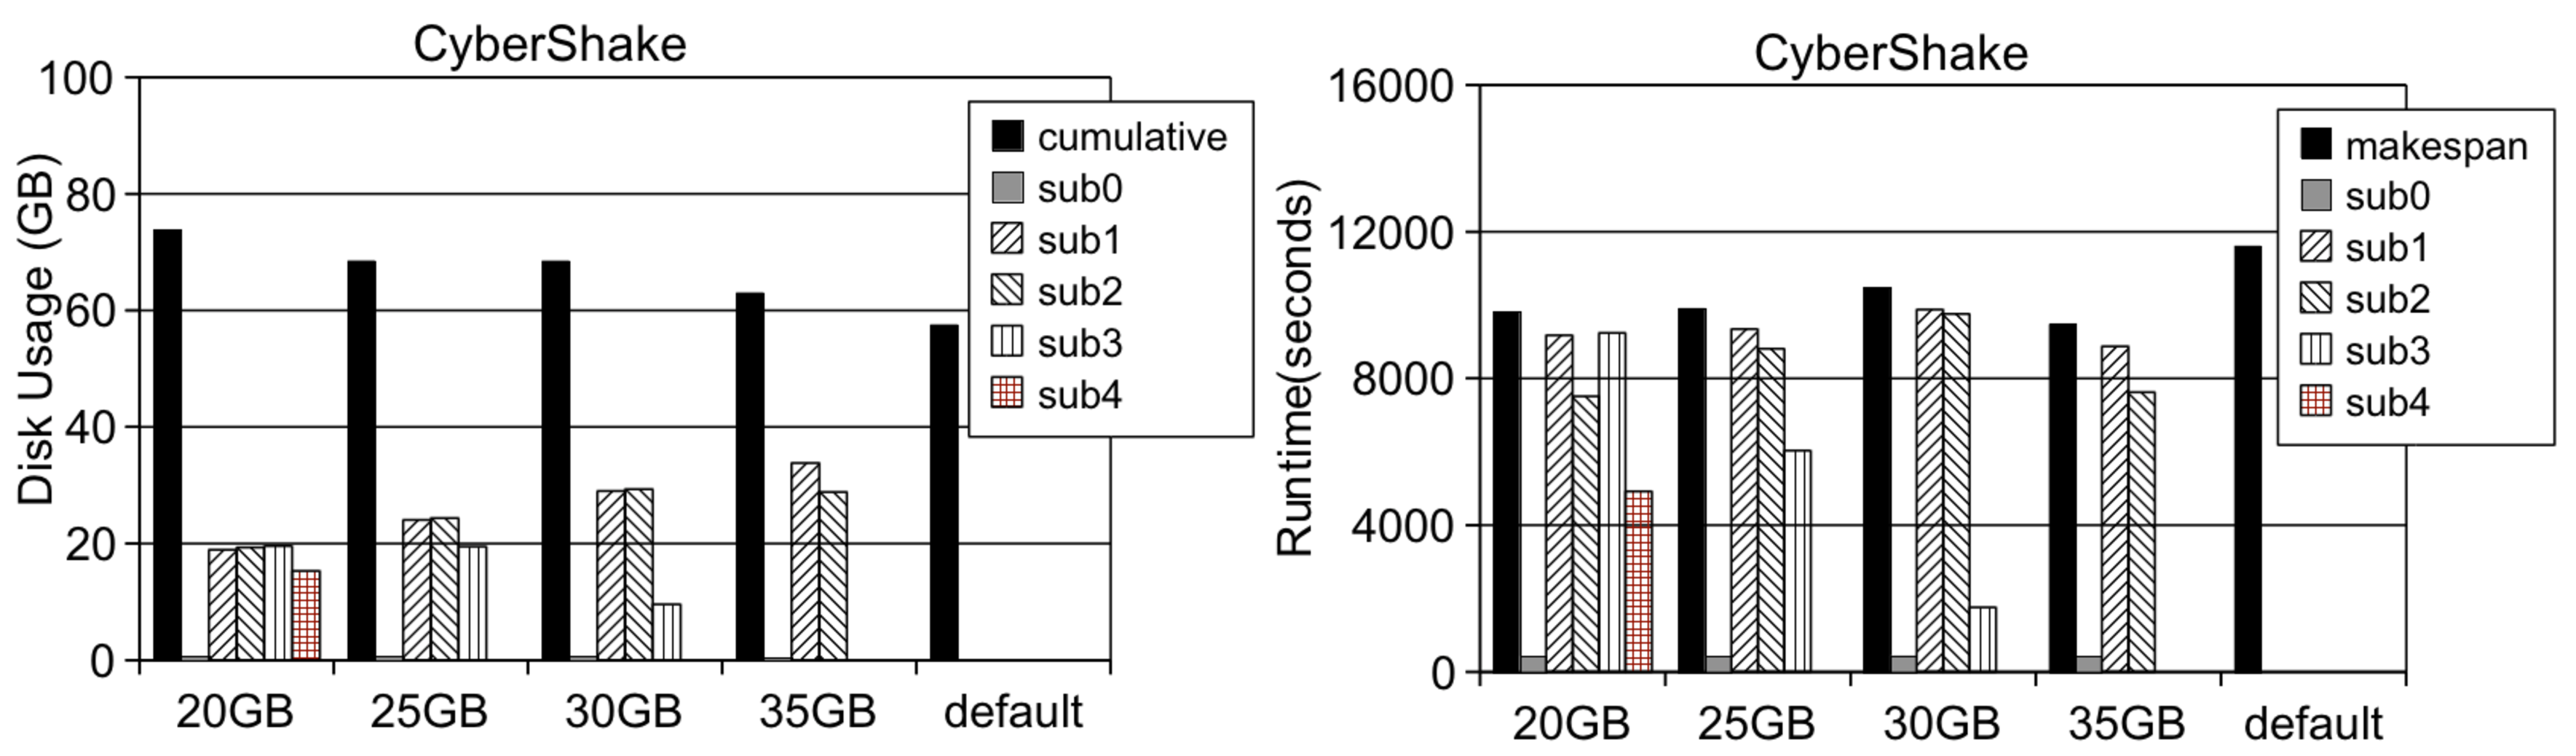
\includegraphics[width=0.9\textwidth]{figures/partitioning/cybershake.pdf}
    \caption{Performance of the CyberShake workflow with different storage constraints}
    \label{fig:cybershake}
\end{figure}

\begin{figure}[h!]
	\centering
    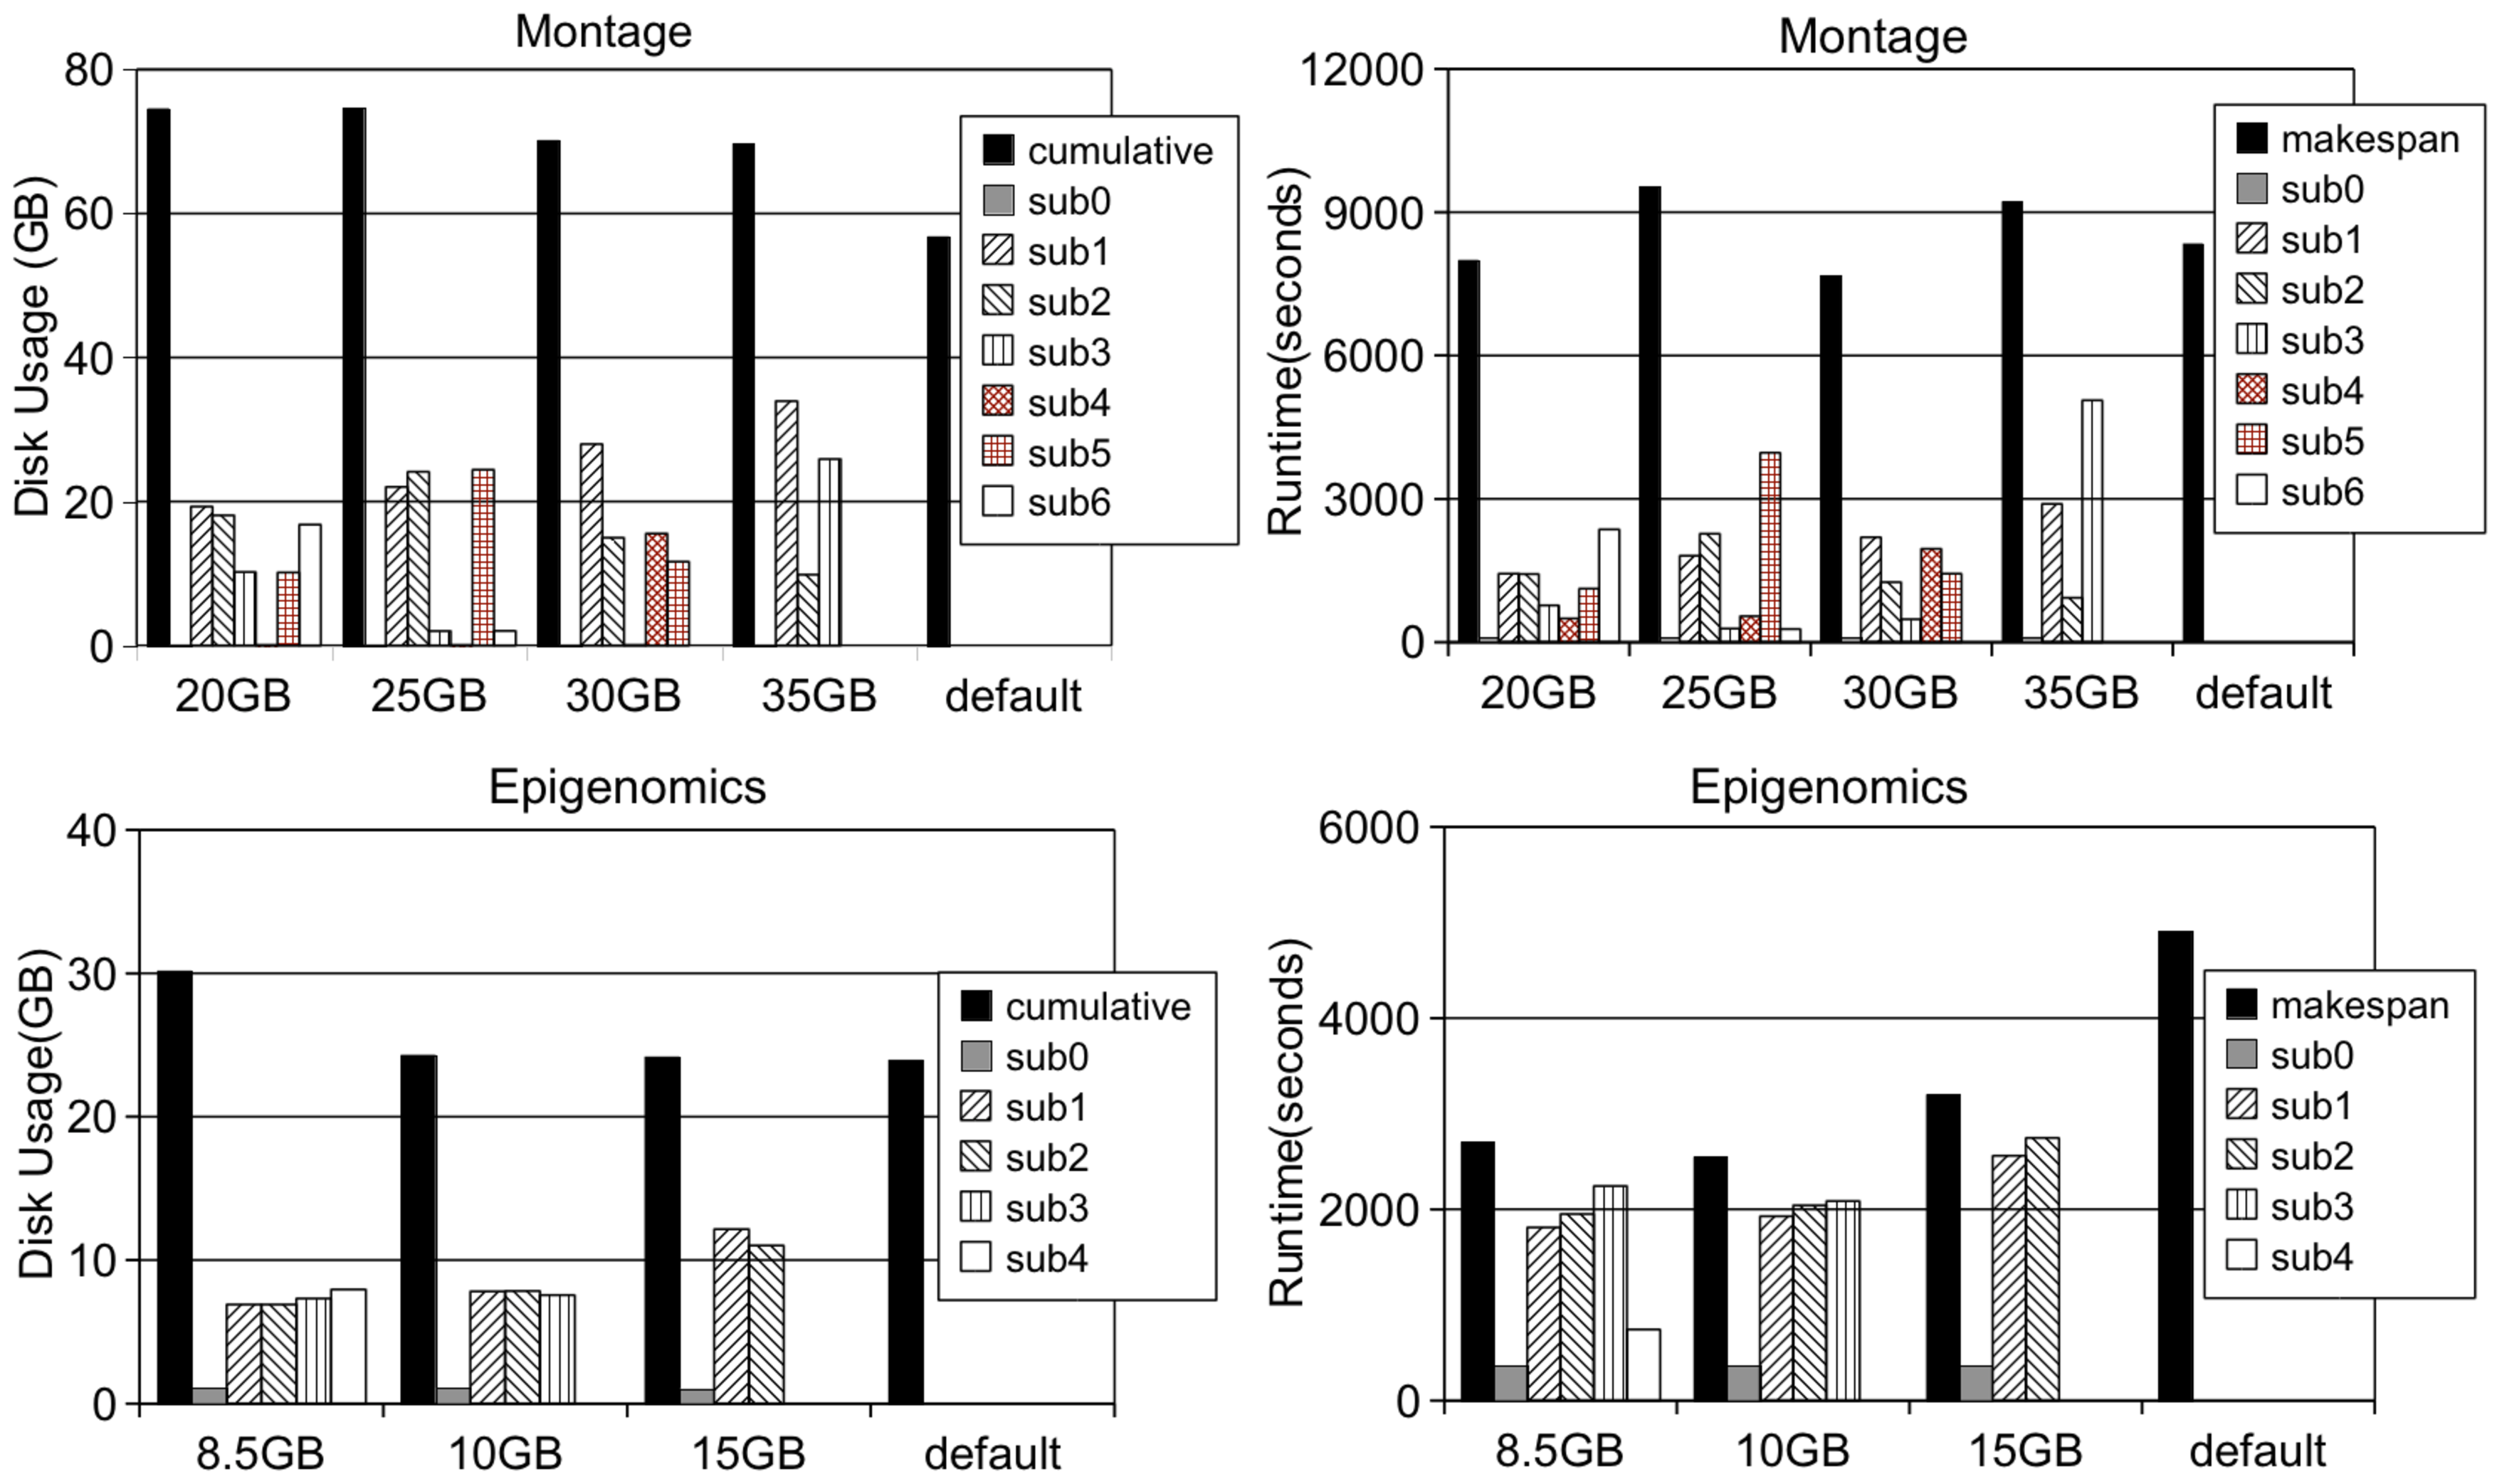
\includegraphics[width=0.9\textwidth]{figures/partitioning/montage2.pdf}
    \caption{Performance of the Montage workflow with different storage constraints}
    \label{fig:montage}
\end{figure}

\textbf{Performance of Different Heuristics}. We compare the three heuristics with the CyberShake application. The storage constraint for each site is 30GB. Heuristic II produces 5 sub-workflows with 10 dependencies between them. Heuristic I produces 4 sub-workflows and 3 dependencies. Heuristic III produces 4 sub-workflows and 5 dependencies. The results are shown in Figure~\ref{fig:heuristics} and Heuristic I performs better in terms of both runtime reduction and disk usage. This is due to the way it handles the cross dependency. Heuristic II or Heuristic III simply adds a job if it does not violate the storage constraints or the cross dependency constraints. Furthermore, Heuristic I puts the entire fan structure into the same sub-workflow if possible and therefore reduces the dependencies between sub-workflows. 
%In Figure~\ref{fig:three_heuristics} with an example of a simplified CyberShake workflow, Heuristic I runs two sub-workflows in parallel while the other two have to run them in sequence. 
From now on, we only use Heuristic I in the partitioner in our experiments below.  

\begin{figure}[h!]
	\centering
    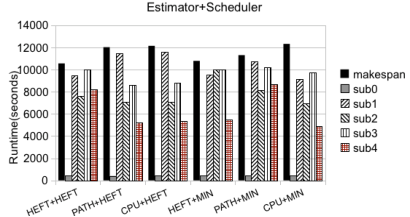
\includegraphics[width=0.7\textwidth]{figures/partitioning/scheduler.pdf}
    \caption{Performance of estimators and schedulers}
    \label{fig:scheduler}
\end{figure}

\begin{table}[h!]
\caption{Performance of estimators and schedulers}
\label{tab:scheduler}
\centering
\begin{tabular}{lrrrr}
\hline
Combination     &     Estimator &     Scheduler &    Makespan(second)  \\
\hline
HEFT+HEFT & HEFT & HEFT & 10559.5\\
PATH+HEFT & Critical Path & HEFT & 12025.4\\
CPU+HEFT & Average CPU Time & HEFT & 12149.2\\
HEFT+MIN & HEFT & MinMin & 10790 \\
PATH+MIN & Critical Path & MinMin & 11307.2 \\
CPU+MIN & Average CPU Time & MinMin & 12323.2\\
\hline
\end{tabular}
\end{table} 

\textbf{Performance with Different Storage Constraints}. Figure~\ref{fig:constraint} and Table~\ref{tab:constraint} depict the disk usage of the CyberShake workflows over time with storage constraints of 35GB, 30GB, 25GB, and 20GB. They are chosen because they represent a variety of required execution sites. Figure~\ref{fig:cybershake} depicts the performance of both disk usage and runtime. Storage constraints for all of the sub-workflows are satisfied. Among them sub1, sub2, sub3 (if exists), and sub4 (if exists) are run in parallel and then sub0 aggregates their work. The CyberShake workflow across two sites with a storage constraint of 35GB performs best. The makespan (overall completion time) improves by 18.38\% and the cumulative disk usage increases by 9.5\% compared to the default workflow without partitioning or storage constraints. The cumulative data usage is increased because some shared data is transferred to multiple sites. Workflows with more sites to run on do not have a smaller makespan because they require more data transfer even though the computation part is improved. 

Figure~\ref{fig:montage} depicts the performance of Montage with storage constraints ranging from 20GB to 35GB and Epigenomics with storage constraints ranging from 8.5GB to 15GB. The Montage workflow across three sites with 30GB disk space performs best with 8.1\% improvement in makespan and the cumulative disk usage increases by 23.5\%. The Epigenomics workflow across three sites with 10GB storage constraints performs best with 48.1\% reduction in makespan and only 1.4\% increase in cumulative storage. The reason why Montage performs worse is related to its complex internal structures. Montage has two levels of fan-out-fan-in structures and each level has complex dependencies between them.
% as shown in Figure~\ref{fig:workflow}. Our heuristic is not able to untie them thoroughly and therefore the cost of data transfer increases and the sub-workflows are not able to run in parallel.

\textbf{Site selection}. To show the performance of site selection for each sub-workflow, we use three estimators and two schedulers  together with the CyberShake workflow. We build four execution sites with 4, 8, 10 and 10 Condor slots respectively. The labels in Figure~\ref{fig:scheduler} and Table~\ref{tab:scheduler} are defined in a way of ‘Estimator + Scheduler’. For example, HEFT+HEFT denotes a combination of HEFT estimator and HEFT scheduler, which performs best as we expected. The Average CPU Time (or ‘CPU’ in Figure 4.7) does not take the dependencies into consideration and the Critical Path (or ‘PATH’ in Figure~\ref{fig:scheduler}) does not consider the resource availability. The HEFT scheduler is slightly better than MinMin scheduler (or ‘MIN’ in Figure~\ref{fig:scheduler}). Although HEFT scheduler uses a global optimization algorithm compared to MinMin’s local optimization, the complexity of scheduling sub-workflows has been greatly reduced compared to scheduling a vast number of individual tasks. Therefore, both local and global optimization algorithms are able to handle such situations well.

In conclusion, we provide a solution to address the problem of scheduling large workflows across multiple sites with storage constraints. The approach relies on partitioning the workflow into valid sub-workflows. Three heuristics are proposed and compared to show the close relationship between cross dependency and runtime improvement. The performance with three workflows shows that this approach is able to satisfy the storage constraints and reduce the makespan significantly especially for Epigenomics which has fewer fan-in (synchronization) jobs. For the workflows we used, scheduling them onto two or three execution sites is best due to a tradeoff between increased data transfer and increased parallelism. Site selection shows that the global optimization and local optimization perform almost the same.  

\section{Summary}

for other constraints

